\subsection{Verso la convergenza tecnologica}
Se vogliamo individuare la causa principale che spinge il meccanismo di innovazione possiamo trovarla nella convergenza tecnologica, ossia il superamento della demarcazione tra mezzi e servizi. 

La branca del diritto che si occupa di questo settore è detta ``diritto della convergenza". 

Durante gli anni '90 si è assistito a numerosi cambiamenti a livello europeo e italiano. La parola telecomunicazioni è presente nella normativa sia italiana che internazionale già nella Convenzione Internazionale di Madrid del 1932. Per telecomunicazioni si intende dunque, tradizionalmente:

\begin{quote}
    Ogni emissione, trasmissione o ricezione di segni, segnali, scritti, immagini, suoni e informazioni di qualsiasi natura, per filo, radioelettrica, ottica o a mezzo di altri sistemi elettromagnetici.    
\end{quote}
(Convenzione Internazionale Madrid 1932, Buenos Aires 1952)

In questa definizione è insita una notevole demarcazione tra i mezzi e i servizi e questo permette alla legislazione che va dagli anni Venti fino alla metà degli anni Ottanta di distinguere strettamente tra mezzi e servizi. 
In un decreto del '73 che regola il codice postale e delle telecomunicazioni si distingue infatti tra:
\begin{itemize}
    \item Telegrafia (via filo)
    \item Telefonia (via filo)
    \item Radiocomunicazioni (onde radio): comprendenti radiodiffusione, radiotelefonia e radiotelegrafia
\end{itemize}

Per gli ambiti di comunicazione One-to-One e comunicazioni broadcast si svilupparono di conseguenza ambiti del diritto distinti.

\begin{figure}
    \centering
    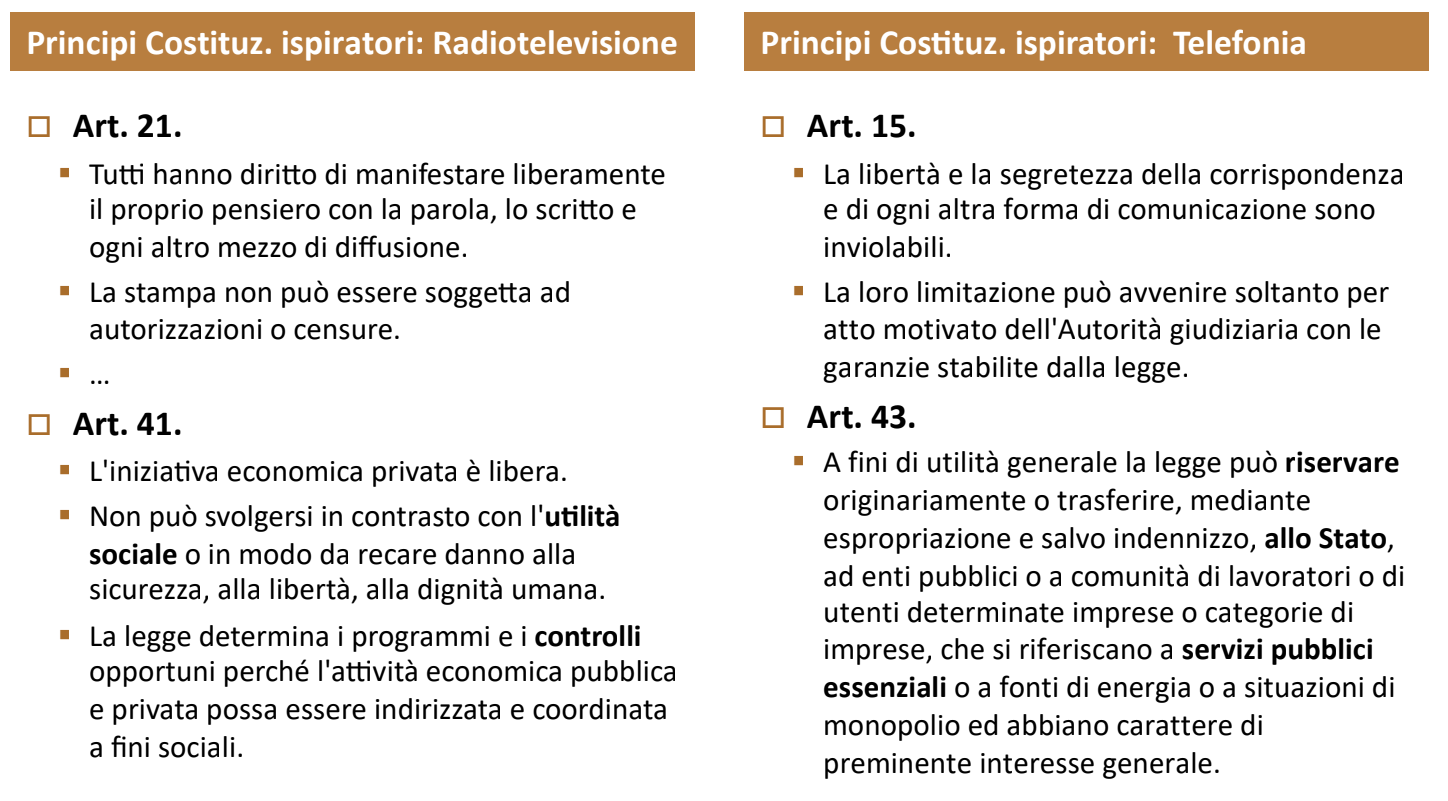
\includegraphics[width=\textwidth]{principi costituzionali.png}
    \caption{Principi costituzionali ispiratori}
\end{figure}

Definiamo \textit{convergenza tecnologica} l'utilizzo stesso mezzo per fornire una pluralità di servizi.

I principali passaggi dell'innovazione tecnologica sono storicamente legati all'avvento della multimedialità:
\begin{itemize}
    \item Telematica: unione tra le TLC e informatica (trasmissione + elaborazione a distanza): l'utente può interagire con l'informazione (anche semplicemente la possibilità di interagire con un televisore tramite telecomando rendendo il servizio non più unidirezionale)
    \item Innovazione e potenziamento dei servizi trasmissivi (fibra, satellite, radiomobile): fruibilità e/o capacità trasmissive notevolmente migliorate
    \item Rappresentazione numerica dell'informazione (segnali): stessa infrastruttura per rappresentare in binario segnali provenienti da diverse sorgenti di informazioni
    \item Sviluppo di tecniche di codifica di sorgente (standard di compressione): riduzione del numero di bit da trasmettere
    \item Tecniche di codifica di canale: affidabilità maggiore della telecomunicazione, riduzione degli errori di trasmissione
    \item Tecniche di crittografia, autenticazione, firma digitale, blockchain: sicurezza, segretezza, autenticazione, privacy, servizi innovativi (es. posta elettronica certificata)
    \item Multimedialità: diverse sorgenti combinate in diversi servizi multimediali su diversi mezzi di tlc collegati attraverso diversi canali di comunicazione in una tendenza alla convergenza di contenuti e servizi su medesime infrastrutture di telecomunicazione
\end{itemize}

Si rese necessario ridefinire delle normative che tenessero conto della multimedialità. 
